\begin{frame}
	\frametitle{Vegetation}

	\begin{figure}
		\centering
		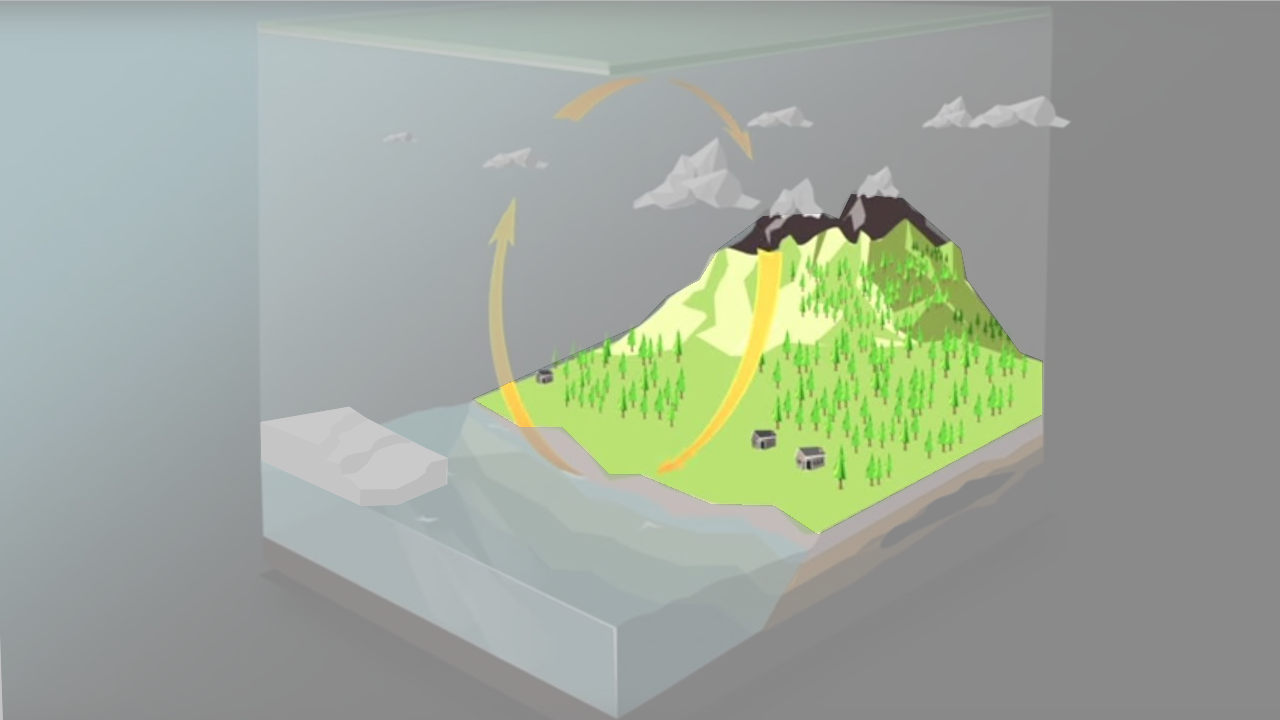
\includegraphics{bilder/WMO_Cycles_land.png}
		\caption{Die Vegetation ist eine interaktive Komponente des Klimasystems}
	\end{figure}

	\note{
		\begin{itemize}
			\item[] Vegetation ist sehr umfangreich und vielseitig
			\item[] steht in direktem Kontakt mit unterer Atmosphäre und Böden
			\item[] durch photosynthetische Prozesse und die Aufnahme sowie Abgabe von Wasser
			\item[] Vegetation hat dadurch massiven Einfluss auf Wetter und Klima - z.B. Tropischer Regenwald, Wolkenbildung
			\item[] zentral ist auch die Rolle beim Stoffkreislauf - u.a. Kohlenstoff, Phosphor, Nitrat, Stickstoff
			\item[] bietet Lebensraum und Lebensgrundlage
		\end{itemize}
	}
\end{frame}
